\documentclass[]{book}
\usepackage{lmodern}
\usepackage{amssymb,amsmath}
\usepackage{ifxetex,ifluatex}
\usepackage{fixltx2e} % provides \textsubscript
\ifnum 0\ifxetex 1\fi\ifluatex 1\fi=0 % if pdftex
  \usepackage[T1]{fontenc}
  \usepackage[utf8]{inputenc}
\else % if luatex or xelatex
  \ifxetex
    \usepackage{mathspec}
  \else
    \usepackage{fontspec}
  \fi
  \defaultfontfeatures{Ligatures=TeX,Scale=MatchLowercase}
\fi
% use upquote if available, for straight quotes in verbatim environments
\IfFileExists{upquote.sty}{\usepackage{upquote}}{}
% use microtype if available
\IfFileExists{microtype.sty}{%
\usepackage{microtype}
\UseMicrotypeSet[protrusion]{basicmath} % disable protrusion for tt fonts
}{}
\usepackage[margin=1in]{geometry}
\usepackage{hyperref}
\hypersetup{unicode=true,
            pdftitle={Statistik},
            pdfauthor={Thomas Petersen},
            pdfborder={0 0 0},
            breaklinks=true}
\urlstyle{same}  % don't use monospace font for urls
\usepackage{natbib}
\bibliographystyle{apalike}
\usepackage{color}
\usepackage{fancyvrb}
\newcommand{\VerbBar}{|}
\newcommand{\VERB}{\Verb[commandchars=\\\{\}]}
\DefineVerbatimEnvironment{Highlighting}{Verbatim}{commandchars=\\\{\}}
% Add ',fontsize=\small' for more characters per line
\usepackage{framed}
\definecolor{shadecolor}{RGB}{248,248,248}
\newenvironment{Shaded}{\begin{snugshade}}{\end{snugshade}}
\newcommand{\AlertTok}[1]{\textcolor[rgb]{0.94,0.16,0.16}{#1}}
\newcommand{\AnnotationTok}[1]{\textcolor[rgb]{0.56,0.35,0.01}{\textbf{\textit{#1}}}}
\newcommand{\AttributeTok}[1]{\textcolor[rgb]{0.77,0.63,0.00}{#1}}
\newcommand{\BaseNTok}[1]{\textcolor[rgb]{0.00,0.00,0.81}{#1}}
\newcommand{\BuiltInTok}[1]{#1}
\newcommand{\CharTok}[1]{\textcolor[rgb]{0.31,0.60,0.02}{#1}}
\newcommand{\CommentTok}[1]{\textcolor[rgb]{0.56,0.35,0.01}{\textit{#1}}}
\newcommand{\CommentVarTok}[1]{\textcolor[rgb]{0.56,0.35,0.01}{\textbf{\textit{#1}}}}
\newcommand{\ConstantTok}[1]{\textcolor[rgb]{0.00,0.00,0.00}{#1}}
\newcommand{\ControlFlowTok}[1]{\textcolor[rgb]{0.13,0.29,0.53}{\textbf{#1}}}
\newcommand{\DataTypeTok}[1]{\textcolor[rgb]{0.13,0.29,0.53}{#1}}
\newcommand{\DecValTok}[1]{\textcolor[rgb]{0.00,0.00,0.81}{#1}}
\newcommand{\DocumentationTok}[1]{\textcolor[rgb]{0.56,0.35,0.01}{\textbf{\textit{#1}}}}
\newcommand{\ErrorTok}[1]{\textcolor[rgb]{0.64,0.00,0.00}{\textbf{#1}}}
\newcommand{\ExtensionTok}[1]{#1}
\newcommand{\FloatTok}[1]{\textcolor[rgb]{0.00,0.00,0.81}{#1}}
\newcommand{\FunctionTok}[1]{\textcolor[rgb]{0.00,0.00,0.00}{#1}}
\newcommand{\ImportTok}[1]{#1}
\newcommand{\InformationTok}[1]{\textcolor[rgb]{0.56,0.35,0.01}{\textbf{\textit{#1}}}}
\newcommand{\KeywordTok}[1]{\textcolor[rgb]{0.13,0.29,0.53}{\textbf{#1}}}
\newcommand{\NormalTok}[1]{#1}
\newcommand{\OperatorTok}[1]{\textcolor[rgb]{0.81,0.36,0.00}{\textbf{#1}}}
\newcommand{\OtherTok}[1]{\textcolor[rgb]{0.56,0.35,0.01}{#1}}
\newcommand{\PreprocessorTok}[1]{\textcolor[rgb]{0.56,0.35,0.01}{\textit{#1}}}
\newcommand{\RegionMarkerTok}[1]{#1}
\newcommand{\SpecialCharTok}[1]{\textcolor[rgb]{0.00,0.00,0.00}{#1}}
\newcommand{\SpecialStringTok}[1]{\textcolor[rgb]{0.31,0.60,0.02}{#1}}
\newcommand{\StringTok}[1]{\textcolor[rgb]{0.31,0.60,0.02}{#1}}
\newcommand{\VariableTok}[1]{\textcolor[rgb]{0.00,0.00,0.00}{#1}}
\newcommand{\VerbatimStringTok}[1]{\textcolor[rgb]{0.31,0.60,0.02}{#1}}
\newcommand{\WarningTok}[1]{\textcolor[rgb]{0.56,0.35,0.01}{\textbf{\textit{#1}}}}
\usepackage{longtable,booktabs}
\usepackage{graphicx,grffile}
\makeatletter
\def\maxwidth{\ifdim\Gin@nat@width>\linewidth\linewidth\else\Gin@nat@width\fi}
\def\maxheight{\ifdim\Gin@nat@height>\textheight\textheight\else\Gin@nat@height\fi}
\makeatother
% Scale images if necessary, so that they will not overflow the page
% margins by default, and it is still possible to overwrite the defaults
% using explicit options in \includegraphics[width, height, ...]{}
\setkeys{Gin}{width=\maxwidth,height=\maxheight,keepaspectratio}
\IfFileExists{parskip.sty}{%
\usepackage{parskip}
}{% else
\setlength{\parindent}{0pt}
\setlength{\parskip}{6pt plus 2pt minus 1pt}
}
\setlength{\emergencystretch}{3em}  % prevent overfull lines
\providecommand{\tightlist}{%
  \setlength{\itemsep}{0pt}\setlength{\parskip}{0pt}}
\setcounter{secnumdepth}{5}
% Redefines (sub)paragraphs to behave more like sections
\ifx\paragraph\undefined\else
\let\oldparagraph\paragraph
\renewcommand{\paragraph}[1]{\oldparagraph{#1}\mbox{}}
\fi
\ifx\subparagraph\undefined\else
\let\oldsubparagraph\subparagraph
\renewcommand{\subparagraph}[1]{\oldsubparagraph{#1}\mbox{}}
\fi

%%% Use protect on footnotes to avoid problems with footnotes in titles
\let\rmarkdownfootnote\footnote%
\def\footnote{\protect\rmarkdownfootnote}

%%% Change title format to be more compact
\usepackage{titling}

% Create subtitle command for use in maketitle
\providecommand{\subtitle}[1]{
  \posttitle{
    \begin{center}\large#1\end{center}
    }
}

\setlength{\droptitle}{-2em}

  \title{Statistik}
    \pretitle{\vspace{\droptitle}\centering\huge}
  \posttitle{\par}
    \author{Thomas Petersen}
    \preauthor{\centering\large\emph}
  \postauthor{\par}
      \predate{\centering\large\emph}
  \postdate{\par}
    \date{2019-04-28}

\usepackage{booktabs}
\usepackage{amsthm}
\makeatletter
\def\thm@space@setup{%
  \thm@preskip=8pt plus 2pt minus 4pt
  \thm@postskip=\thm@preskip
}
\makeatother

\begin{document}
\maketitle

{
\setcounter{tocdepth}{1}
\tableofcontents
}
\hypertarget{section}{%
\chapter*{}\label{section}}
\addcontentsline{toc}{chapter}{}

\hypertarget{Settings}{}

\hypertarget{TopBar}{}
\hypertarget{Sentry_label}{}
\protect\hypertarget{Sentry_label_span}{}{Adgang}\protect\hypertarget{downArrow}{}{}

\hypertarget{magicGroup}{}
\hypertarget{messages}{}
.

\leavevmode\hypertarget{Sentry_emailDiv}{}%

\hypertarget{Sentry_passwordDiv}{}
{
}

\hypertarget{Sentry_HIDpasswordDiv}{}
{
}

\hypertarget{unHideDiv}{}
\protect\hypertarget{forgotSpan}{}{Glemt?}
\protect\hypertarget{unHideSpan}{}{Vis}

\hypertarget{buttonDiv}{}
Login her!

\hypertarget{psistDiv}{}

\hypertarget{psistDiv}{}
\protect\hypertarget{psistSpan}{}{Husk mig}

\hypertarget{goInside}{}
\protect\hypertarget{goInsideSpan}{}{.}

\hypertarget{signUp}{}
\hypertarget{psistDiv}{}

\hypertarget{signUp}{}
\hypertarget{psistDiv}{}

\hypertarget{signUp}{}
Profil/Afmeld

\hypertarget{psistDiv}{}

\hypertarget{logOut}{}
{Log ud}

\hypertarget{xbox}{}

\hypertarget{Sentry_noJSLogin}{}
{Javascript Required}

\hypertarget{Sentry_loggingIn}{}

\hypertarget{Sentry_In}{}
For testing.

You must have JavaScript enabled in order to log in.

Video sådan køber du adgang.

Video sådan logger du ind.

Use \texttt{gitbook} to convert the \texttt{text} in markdown
syntax to HTML.

\hypertarget{indledning}{%
\chapter{Indledning}\label{indledning}}

\hypertarget{Sentry_noJS}{}
Sentry Page Protection

\hypertarget{Sentry_redirecting}{}
Please Wait\ldots{}

Dette er undervisningsmateriale og opgaver til faget statistik, for erhvervsakademierne.

Orley Ashenfelter en Princeton økonom udviklede i 1980'erne en statistik model til forudsigelse af vinpriser baseret på nedbør, solskinstimer og andre klimadata. Hele den etablerede vinverden var i oprør, ved en præsentation i Christie's vinafdeling, blev han buhet ud. Robert Parker den verdenskendte vinkender udtalte ``Det svarer til en filmanmelder der ikke ser filmen, men udelukkende baserer sin anmeldelse på instruktøren og skuespilleren''. Orley udtalte, lang tid før det var muligt for vinseksperterne, at 1989 Bordeux ville blive århundredets vin, uanset den kun havde ligget 3 måneder på fade. Flere analyser har siden vist Orleys model er langt mere præcis eksperterne. Meget få vinkendere har anerkendt kvaliteten af Orleys model, men deres forecasts ligger nu langt tættere på modellens forudsigelser.

Bogen er opbygget med en del praktiske eksempler.

Der er i nogle afsnit knapper med spørgsmål og svar, man kan klikke på disse og se om man kan nå frem til de rigtige løsninger.

Bogen er bygget op så kapitlerne beskriver fanerne i Freestat programmet. Man kan se og hente excelfiler direkte ved at klikke på links.

I alle brancher i den finansielle sektor spiller statistik en rolle.

Bankerne sammensætter investeringsporteføljer, der minimerer risikoen (variansen), ved aktiver der har lav eller negativ samvariation (kovarians). Cykliske aktier som FL Smidth har fx. lav samvariation med en ikke cyklisk aktie som Novo.

Forsikringsselskaberne beregner præmier for forsikringstageren, baseret på statistike sandsynligheder for at en hændelse indtræffer. Modellerne kan være meget specifikke, en indboforsikring kan fx. være baseret på ikke bare postnummer, boligform, men også etage.

Finansielle virksomheder underlagt finanstilsynet, bruger modeller til beregning af risiko baseret på statistisk analyse.

Mægleren beregner udbudspriser, udfra en multipel lineær regressionsmodel, der indeholder variable som størrelse, energimærke, tagtype etc.

\hypertarget{freestat-basisversion}{%
\section{Freestat basisversion}\label{freestat-basisversion}}

Man kan få beregnet deskriptorerne i et utal af programmer heriblandt Freestat basis et gratis program, der kan hentes ved at \href{https://www.dropbox.com/s/th8q95lf864npie/FREESTATfin.xlsx?dl=1}{klikke her.} Freestat basis, kan gennemføre de mest almindelige statistiske analyser.

\hypertarget{freestat-fuld-version}{%
\section{Freestat fuld version}\label{freestat-fuld-version}}

Har du købt adgang til premium abbonnementet, er der en del ekstra analyser, derfor bør du hente Freestat premium versionen. Seneste version af programmet kan \href{https://www.dropbox.com/s/a2jztexbxfzcli0/FREESTAT.xlsx?dl=1}{hentes her.}

Du kan finde flere resourcer bagerst i bogen under materialer ved at \href{https://s.tepedu.dk/materialer.html}{klikke her.}

Der findes opgaver quizzes og yderligere resourcer på \href{http://www.edutest.dk}{www.edutest.dk}

Min gode ven Benjamin Tejlbjerg har lavet en super hjemmeside med gymnasie matematik og statistik \href{http://www.mathhx.dk/?q=node/117}{http://www.mathhx.dk}. Siden er gratis og god til at genopfriske basisbegreber indenfor statistik, vi kommer ikke i dybden med disse begreber her.

Denne online bog rettes og opdateres løbende med nye videoer opgaver og quizzes, der tages forbehold for tryk og tastefejl, men alle fejl eller uklarheder I måtte finde rettes med fluks. Forslag til forbedringer modtages med kyshånd.

\textbf{\emph{Noterne er kun til personligt brug. Alle rettigheder forbeholdes. Fotografisk eller anden gengivelse af eller kopiering eller anden udnyttelse, er uden forfatterens skriftlige samtykke forbudt ifølge dansk lov om ophavsret.}}

\hypertarget{datast-og-data}{%
\chapter{Datasæt og data}\label{datast-og-data}}

\hypertarget{Sentry_noJS}{}
Sentry Page Protection

\hypertarget{Sentry_redirecting}{}
Please Wait\ldots{}

\hypertarget{uni--bi--og-multivariate-datast}{%
\subsection{Uni- bi- og multivariate datasæt}\label{uni--bi--og-multivariate-datast}}

Datasæt er sæt af en eller flere variable:

\begin{itemize}
\tightlist
\item
  Univariate datasæt fx tider ved marathonløb\\
\item
  Bivariate datasæt fx tider ved marathonløb og køn
\item
  Multivariate datasæt fx tider ved marathonløb, køn, alder, medlem af sports klub
\end{itemize}

\hypertarget{kvalitative-variable}{%
\subsection{Kvalitative variable}\label{kvalitative-variable}}

Kvalitative variable er data vi ikke kan måle eller tælle. De antager værdier i form af navne eller labels:

\begin{itemize}
\tightlist
\item
  Kæledyr: kat, hund, marsvin
\item
  Køn: mand, kvinde
\item
  Favorit app: Angry Birds, Messenger, Audible, Tinder
\end{itemize}

\hypertarget{kvantitative-variable}{%
\subsection{Kvantitative variable}\label{kvantitative-variable}}

Kvantitative variable er målbare numeriske variable, vi deler disse op i \emph{kontinuerte} og \emph{diskrete} variable

\hypertarget{diskrete-variable}{%
\subsubsection{Diskrete variable}\label{diskrete-variable}}

Diskrete variable er fx.

\begin{itemize}
\tightlist
\item
  Antal biler der passerer en bro observeret over flere dage.
\item
  Dagsproduktionen af chokoladefrøer på Toms.
\item
  Antal personer der har iphones
\item
  Antallet af indbyggere i en by
\end{itemize}

\hypertarget{kontinuerte-variable}{%
\subsubsection{Kontinuerte variable}\label{kontinuerte-variable}}

Kontinuerte variable er fx.

\begin{itemize}
\tightlist
\item
  Antal ml. indhold i shampoo flasker
\item
  Aktiekurser for Intel
\item
  Vægten på værnepligtige
\item
  Højden på studerende
\end{itemize}

\hypertarget{skalatyper}{%
\subsection{Skalatyper}\label{skalatyper}}

Vi kan ydermere inddele variable efter skalatype hvor lavere betyder mindst restriktiv.

\begin{enumerate}
\def\labelenumi{\arabic{enumi}.}
\tightlist
\item
  Nominalskala, bruges til at måle kvalitative data (er der kun 2 mulige udfald kaldes variablen specielt binær eller dikotom), fx.

  \begin{itemize}
  \tightlist
  \item
    Køn Mand Kvinde\\
  \item
    Styresystem: IOS Android Windows Symbian Andet
  \item
    Race: Europæisk, Afrikansk, Asiatisk Andet
  \end{itemize}
\item
  Ordinalskala inddeler data efter en rangordning

  \begin{itemize}
  \tightlist
  \item
    Karakterer på 7 trins skalaen -3 00 02\ldots{}
  \item
    Moodys credit ratings Aaa Aa A Baa Ba B Caa Ca C
  \item
    Tilfredshed meget utilfreds, noget utilfreds, nogenlunde tilfreds, meget tilfreds
  \end{itemize}
\item
  Intervalskala man kan sammenligne afstande og forskelle, men der er intet meningsfuldt nulpunkt. Nul for en intervalskala variabel betyder således ikke fravær af den målte størrelse. Nul grader celsius betyder altså ikke fravær af temperatur (det absolutte nulpunkt 0 Kelvin, hvor alle molekyler og atomer er i grundtilstanden). En IQ på 0 betyder ikke fravær af intelligens.

  \begin{itemize}
  \tightlist
  \item
    Temperatur målt i Celsius
  \item
    Temperatur målt i Fahrenheit
  \item
    PH
  \item
    IQ
  \end{itemize}
\item
  Ratioskala

  \begin{itemize}
  \tightlist
  \item
    Beløb i lommen
  \item
    Højde på studerende
  \item
    Hastighed af biler ved vejkryds
  \item
    Indhold i Coca Cola flasker
  \end{itemize}
\end{enumerate}

``Statistics are used much like a drunk uses a lamppost: for support, not illumination.''\\
- Vin Scully

Interval- og ratioskalaer omtales som numeriske eller kontinuerte skalaer, disse er knyttet til kvantitative variable.\\
Nominal- og ordinalskalaer omtales ofte som kategorisk eller faktor, disse er knyttet til kvalitative variable.

En stikprøve af skalatype ratio kan fx. reduceres til ordinal, eller nominal. Temperatur målt i celsius kan fx. omskrives til en ordinal variabel: koldt normalt varmt, eller en nominal variabel: ekstrem temperatur eller normal temperatur.

Kategoriske skalaer kan yderligere reduceres til en dikotom skala, ved at sammenlægge kategorierne, til man kun har 2 kategorier.

Det er vanskeligere at ændre en nominal- ordinal- eller ratioskala til en intervalskala. At ændre variablen nominalskala variablen køn til ordinal giver fx. ikke mening.

\hypertarget{materialer}{%
\chapter{Materialer}\label{materialer}}

\hypertarget{Sentry_noJS}{}
Sentry Page Protection

\hypertarget{Sentry_redirecting}{}
Please Wait\ldots{}

\begin{longtable}[]{@{}l@{}}
\toprule
MINDMAPS og Freestat\tabularnewline
\midrule
\endhead
\href{https://www.dropbox.com/s/a2jztexbxfzcli0/FREESTAT.xlsx?dl=1}{Hent Freestat premium her}\tabularnewline
\href{https://www.dropbox.com/s/th8q95lf864npie/FREESTATfin.xlsx?dl=1}{Hent Freestat basis her}\tabularnewline
\href{https://drive.google.com/uc?export=download\&id=0B1E7VnhxsDMlQ1Zhdjh5WTJ4bnM}{CPH Finansøkonom statistik mindmap}\tabularnewline
\bottomrule
\end{longtable}

\begin{center}\rule{0.5\linewidth}{\linethickness}\end{center}

\begin{longtable}[]{@{}l@{}}
\toprule
Skabeloner\tabularnewline
\midrule
\endhead
\href{https://www.dropbox.com/s/xygqhfe6wmxzntf/Skabelon\%20test\%20af\%20middelv\%C3\%A6rdi\%20\%CE\%BC.docx?dl=1}{Skabelon test af middelværdi}\tabularnewline
\href{https://www.dropbox.com/s/m3vmdo47f6ocza3/skabelon\%20test\%20af\%20standardafvigelse.docx?dl=1}{Skabelon test af standardafvigelse}\tabularnewline
\href{https://www.dropbox.com/s/vazc4t384xfw2vf/Skabelon\%20test\%20af\%20andel\%20p.docx?dl=1}{Skabelon test af andel p}\tabularnewline
\href{https://www.dropbox.com/s/wbu8gaasar0i991/Skabelon\%20test\%20af\%202\%20andele.docx?dl=1}{Skabelon test af 2 andele}\tabularnewline
\href{https://www.dropbox.com/s/9qv7i2xlt2ioiut/Skabeloner\%20test\%202\%20middelv\%C3\%A6rdier.docx?dl=1}{Skabeloner test 2 middelværdier}\tabularnewline
\href{https://www.dropbox.com/s/8ppxk89bapfh53p/Skabelon\%20Simpel\%20line\%C3\%A6r\%20regression.docx?dl=1}{Skabelon Simpel lineær regression}\tabularnewline
\href{https://www.dropbox.com/s/jghmkyl4ou66lim/Skabelon\%20Multipel\%20line\%C3\%A6r\%20regression\%20slutmodel.docx?dl=1}{Skabelon Multipel lineær regression}\tabularnewline
\href{https://www.dropbox.com/s/ectavp709wtmv6p/Skabelon\%20Goodness\%20of\%20fit\%20test.docx?dl=1}{Skabelon Goodness of fit test}\tabularnewline
\href{https://www.dropbox.com/s/gc0u8hdyrksa9jw/Skabelon\%20Chi\%20i\%20anden\%20test.docx?dl=1}{Skabelon Chi i anden test}\tabularnewline
\href{https://www.dropbox.com/s/9q9joeo1gv8ywky/Skabelon\%20ANOVA\%3AANAVA.docx?dl=1}{Skabelon ANOVA/ANAVA}\tabularnewline
\bottomrule
\end{longtable}

\begin{center}\rule{0.5\linewidth}{\linethickness}\end{center}

\begin{longtable}[]{@{}l@{}}
\toprule
Datasæt\tabularnewline
\midrule
\endhead
\href{https://drive.google.com/uc?export=download\&id=0B1E7VnhxsDMldkt1OUx6LTEyMXM}{2015-Januar-Data.xlsx}\tabularnewline
\href{https://drive.google.com/uc?export=download\&id=0B1E7VnhxsDMlRlVQcFBtdVlHZ1U}{AFFAIRS.xls data vedr. utroskab}\tabularnewline
\href{https://drive.google.com/uc?export=download\&id=0B1E7VnhxsDMlRENKWWxlNlBXbmM}{BANKDATA.xls data vedr. bankansattes uddannelse, køn og etnicitet}\tabularnewline
\href{https://drive.google.com/uc?export=download\&id=0B1E7VnhxsDMlUGdpNXZjWm1sNk0}{Debt.xlsx}\tabularnewline
\href{https://drive.google.com/uc?export=download\&id=0B1E7VnhxsDMlYTRWVWozb09PRTQ}{Forbes 400 2014 RICH US}\tabularnewline
\href{https://drive.google.com/uc?export=download\&id=0B1E7VnhxsDMlNEdtLUV3NFJTSkk}{Forbes-Global-2000 YEAR 2015}\tabularnewline
\href{https://drive.google.com/uc?export=download\&id=0B1E7VnhxsDMlNTkzeVJlQV81OHM}{FORD FOCUS}\tabularnewline
\href{https://drive.google.com/uc?export=download\&id=0B1E7VnhxsDMlQm51dXNjM3NmdE0}{Fortune-Global-500}\tabularnewline
\href{https://drive.google.com/uc?export=download\&id=0B1E7VnhxsDMlQUhPbEgxdmJhZTg}{GDP}\tabularnewline
\href{https://drive.google.com/uc?export=download\&id=0B1E7VnhxsDMlSVkweHBpT19GZjg}{GDP PER CAPITA USD}\tabularnewline
\href{https://drive.google.com/uc?export=download\&id=0B1E7VnhxsDMlamdFSkk4SWU4eWM}{GDP2015}\tabularnewline
\href{https://drive.google.com/uc?export=download\&id=0B1E7VnhxsDMlMTM1UUNMdzdoUm8}{HELBRED}\tabularnewline
\href{https://drive.google.com/uc?export=download\&id=0B1E7VnhxsDMlS3Y5ZUhROU9iNnM}{Hjemmesidedesigns besøgstider i millisekunder}\tabularnewline
\href{https://drive.google.com/uc?export=download\&id=0B1E7VnhxsDMlWlFNLTVoMEU1WHM}{IMDB stikprøve på 759 film}\tabularnewline
\href{https://drive.google.com/uc?export=download\&id=0B1E7VnhxsDMlalR4TGdjSkV0RzA}{KØNSROLLER}\tabularnewline
\href{https://drive.google.com/uc?export=download\&id=0B1E7VnhxsDMlSTFXM1pCMUtjc2M}{MEDIEFORBRUG}\tabularnewline
\href{https://drive.google.com/uc?export=download\&id=0B1E7VnhxsDMlOWNjUzlQd0s4TVE}{SOMMERHUSE LEJE RØMØ}\tabularnewline
\href{https://drive.google.com/uc?export=download\&id=0B1E7VnhxsDMlRURnNjk0UnJSYzQ}{Statkarakterer}\tabularnewline
\href{https://drive.google.com/uc?export=download\&id=0B1E7VnhxsDMlYWJOOG5yamNoOTQ}{TITANIC}\tabularnewline
\href{https://drive.google.com/uc?export=download\&id=0B1E7VnhxsDMlMFZJdm5QdXpGTGc}{TYVERI}\tabularnewline
\href{https://drive.google.com/uc?export=download\&id=0B1E7VnhxsDMlRDhUYUk4R0NwVFk}{usarrest}\tabularnewline
\href{https://drive.google.com/uc?export=download\&id=0B1E7VnhxsDMlVmxHTDltNk1VSG8}{VIRKSOMHEDER-DK}\tabularnewline
\href{https://drive.google.com/uc?export=download\&id=0B1E7VnhxsDMlYnFpbWp1YTBlLVE}{Yahooinvestexcel}\tabularnewline
\href{https://drive.google.com/uc?export=download\&id=0B1E7VnhxsDMldVZtS2tzV0RqVjQ}{USA afkast pr md}\tabularnewline
\href{https://drive.google.com/uc?export=download\&id=0B1E7VnhxsDMlekM5eVRYZkdUZnc}{Hjemmeopgave USA afkast}\tabularnewline
\href{https://drive.google.com/uc?export=download\&id=0B1E7VnhxsDMlSDNPZi1zSTlqNk0}{Hjemmeopgave USA afkast løsning}\tabularnewline
\bottomrule
\end{longtable}

\begin{center}\rule{0.5\linewidth}{\linethickness}\end{center}

\begin{longtable}[]{@{}l@{}}
\toprule
Finansøkonom valgfag statistik eksamensopgaver\tabularnewline
\midrule
\endhead
\href{https://www.dropbox.com/s/lpiglled5qdmtjh/2017\%20December\%20eksamensopgave\%20valgfag\%20statistik.pdf?dl=1}{2017 December eksamensopgave valgfag statistik}\tabularnewline
\href{https://www.dropbox.com/s/ki9mpbsn8jak84i/2017\%20December\%20-\%20Data.xlsx?dl=1}{2017 December data valgfag statistik}\tabularnewline
\href{https://www.dropbox.com/s/3wwbnvyxdz5z04h/2017\%20November\%20eksamensopgave\%20valgfag\%20statistik.pdf?dl=1}{2017 November eksamensopgave valgfag statistik}\tabularnewline
\href{https://www.dropbox.com/s/nqqyc5puaqjuoo7/2017\%20November\%20valgfag\%20statistik\%20-\%20Erstatninger.xlsx?dl=1}{2017 November data valgfag statistik}\tabularnewline
\href{https://www.dropbox.com/s/hc44wglho5tccgs/2017\%20Juni\%20eksamensopgave\%20valgfag\%20statistik.pdf?dl=1}{2017 Juni eksamensopgave valgfag statistik}\tabularnewline
\href{https://www.dropbox.com/s/73azkke4vnduzbk/2017\%20Juni\%20Data\%20-\%20Billeasing.xlsx?dl=1}{2017 Juni data valgfag statistik}\tabularnewline
\href{https://www.dropbox.com/s/psnsb67bw4v98a7/2017\%20Maj\%20eksamensopgave\%20valgfag\%20statistk.pdf?dl=1}{2017 Maj eksamensopgave valgfag statistik}\tabularnewline
\href{https://www.dropbox.com/s/7wpcnkdrjs9tetl/2017\%20Maj\%20Bank.xlsx?dl=1}{2017 Maj data valgfag statistik}\tabularnewline
\href{https://www.dropbox.com/s/4z84mj0mvx4xrql/2017\%20Maj\%20Valgfag\%2C\%20statistik\%20-\%20l\%C3\%B8sning.docx?dl=1}{2017 Maj løsningsforslag valgfag statistik}\tabularnewline
\bottomrule
\end{longtable}

\begin{center}\rule{0.5\linewidth}{\linethickness}\end{center}

\begin{longtable}[]{@{}l@{}}
\toprule
Finansøkonom statistik eksamensopgaver\tabularnewline
\midrule
\endhead
\href{https://drive.google.com/drive/folders/0B1E7VnhxsDMlUTJXLWowYjFNTzg?usp=sharing}{Mappe med gamle eksamensopgaver}\tabularnewline
\bottomrule
\end{longtable}

\begin{center}\rule{0.5\linewidth}{\linethickness}\end{center}

\begin{longtable}[]{@{}l@{}}
\toprule
Edutest\tabularnewline
\midrule
\endhead
\href{http://www.edutest.dk}{www.edutest.dk}\tabularnewline
\bottomrule
\end{longtable}

\begin{center}\rule{0.5\linewidth}{\linethickness}\end{center}

\begin{longtable}[]{@{}l@{}}
\toprule
Hjemmeside af Benjamin Tejlbjerg med gymnasie matematik og statistik\tabularnewline
\midrule
\endhead
\href{http://www.mathhx.dk/?q=node/117}{http://www.mathhx.dk}\tabularnewline
\bottomrule
\end{longtable}

\hypertarget{arima-af-hjere-orden}{%
\section{ARIMA af højere orden}\label{arima-af-hjere-orden}}

Arima modeller kan afhænge af flere tidligere perioder, fx kan ligningen for ARIMA(2,0,0) eller AR(2), opskrives som:

\[\hat{Y_t}=c + \phi Y_{t-1}+ \phi_2 Y_{t-2}\]
Modellen afhænger altså af 2 tidligere perioder (lags) og ikke en. Man betegner dette som en model med lag 2.

Arima modeller kan indeholde flere forskellige elementer med lag som fx. ARIMA(0,2,1).

\hypertarget{arima-og-ssonalitet}{%
\section{ARIMA og sæsonalitet}\label{arima-og-ssonalitet}}

Hvis fx. en aktie handles lavere om fredagen kan ARIMA modellerne korrigere for dette ved sæsonkorrektion. I sæsonkorrigerede modeller vises dette som en ekstra vektor med 3 tal for hhv. sæsonkorrigeret AR eller SAR, sæsonkorrigeret I eller SI og sæsonkorrigeret MA eller SMA. En model som ARIMA(1,0,0)(1,0,0) har altså udover AR også en sæsonkomponent.

\hypertarget{arima-eksempler}{%
\section{ARIMA eksempler}\label{arima-eksempler}}

\hypertarget{traktorer}{%
\subsection{Traktorer}\label{traktorer}}

Hent følgende data for traktor salg, med følgende kommandoer i R.

\begin{Shaded}
\begin{Highlighting}[]
\NormalTok{data =}\StringTok{ }\KeywordTok{read.csv}\NormalTok{(}\StringTok{'http://ucanalytics.com/blogs/wp-content/uploads/2015/06/Tractor-Sales.csv'}\NormalTok{)}
\NormalTok{data =}\StringTok{ }\KeywordTok{ts}\NormalTok{(data[,}\DecValTok{2}\NormalTok{],}\DataTypeTok{start =} \KeywordTok{c}\NormalTok{(}\DecValTok{2003}\NormalTok{,}\DecValTok{1}\NormalTok{),}\DataTypeTok{frequency =} \DecValTok{12}\NormalTok{)}
\end{Highlighting}
\end{Shaded}

Vi ser salget er voksende over tid, der er ligeledes en sæsonkomponent.

\begin{Shaded}
\begin{Highlighting}[]
\KeywordTok{plot}\NormalTok{(data, }\DataTypeTok{xlab=}\StringTok{'Years'}\NormalTok{, }\DataTypeTok{ylab =} \StringTok{'Tractor Sales'}\NormalTok{)}
\end{Highlighting}
\end{Shaded}

\includegraphics{_main_files/figure-latex/unnamed-chunk-2-1.pdf}

Differens tranformer data for at generere stationære data mht. middel (fjern trend)

\begin{Shaded}
\begin{Highlighting}[]
\KeywordTok{plot}\NormalTok{(}\KeywordTok{diff}\NormalTok{(data),}\DataTypeTok{ylab=}\StringTok{'Differenced Tractor Sales'}\NormalTok{)}
\end{Highlighting}
\end{Shaded}

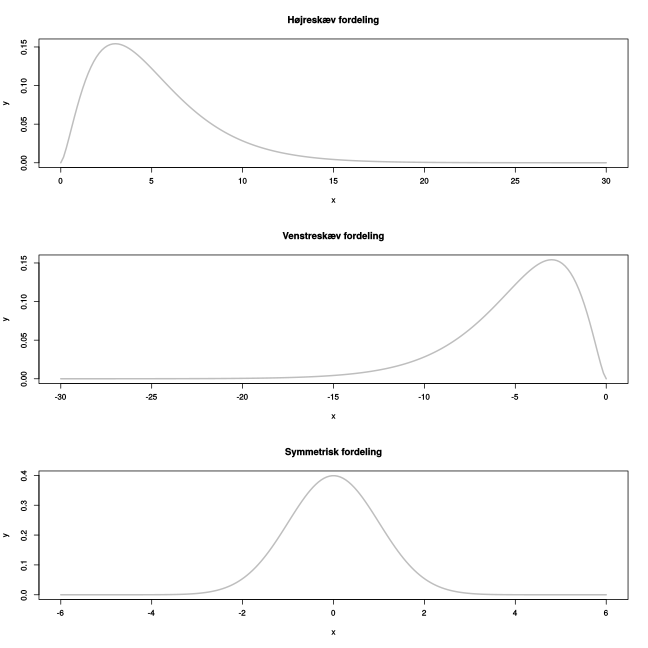
\includegraphics{_main_files/figure-latex/unnamed-chunk-3-1.pdf}

log transformer data for at sikre stationaritet mht. varians.

\begin{Shaded}
\begin{Highlighting}[]
\KeywordTok{plot}\NormalTok{(}\KeywordTok{log10}\NormalTok{(data),}\DataTypeTok{ylab=}\StringTok{'Log (Tractor Sales)'}\NormalTok{)}
\end{Highlighting}
\end{Shaded}

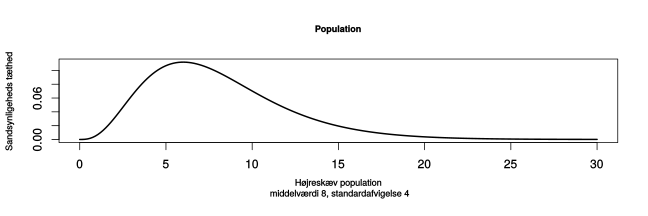
\includegraphics{_main_files/figure-latex/unnamed-chunk-4-1.pdf}

Eventuel Differens og log transformation af data for at sikre stationaritet både mht. middel og varians.

\begin{Shaded}
\begin{Highlighting}[]
\KeywordTok{plot}\NormalTok{(}\KeywordTok{diff}\NormalTok{(}\KeywordTok{log10}\NormalTok{(data)),}\DataTypeTok{ylab=}\StringTok{'Differenced Log (Tractor Sales)'}\NormalTok{)}
\end{Highlighting}
\end{Shaded}

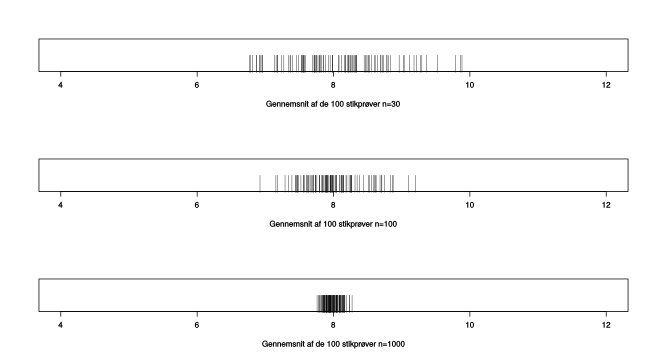
\includegraphics{_main_files/figure-latex/unnamed-chunk-5-1.pdf}

Find bedste model med auto.arima, når der er stationaritet.

Akaike Information Criterion (AIC) , og Bayesian Information Criterion (BIC), vælg ARIMA modellen med mindst AIC and BIC værdier. auto.arima finder den bedste model automatisk.

\begin{Shaded}
\begin{Highlighting}[]
\KeywordTok{require}\NormalTok{(forecast)}
\NormalTok{ARIMAfit =}\StringTok{ }\KeywordTok{auto.arima}\NormalTok{(}\KeywordTok{log10}\NormalTok{(data), }\DataTypeTok{approximation=}\OtherTok{FALSE}\NormalTok{,}\DataTypeTok{trace=}\OtherTok{FALSE}\NormalTok{)}
\NormalTok{ARIMAfit}
\end{Highlighting}
\end{Shaded}

\begin{verbatim}
## Series: log10(data) 
## ARIMA(0,1,1)(0,1,1)[12] 
## 
## Coefficients:
##           ma1     sma1
##       -0.4047  -0.5529
## s.e.   0.0885   0.0734
## 
## sigma^2 estimated as 0.0002571:  log likelihood=354.4
## AIC=-702.79   AICc=-702.6   BIC=-694.17
\end{verbatim}

Nu kan vi forudsige kommende traktor salg med modellen

\begin{Shaded}
\begin{Highlighting}[]
\KeywordTok{par}\NormalTok{(}\DataTypeTok{mfrow =} \KeywordTok{c}\NormalTok{(}\DecValTok{1}\NormalTok{,}\DecValTok{1}\NormalTok{))}
\NormalTok{pred =}\StringTok{ }\KeywordTok{predict}\NormalTok{(ARIMAfit, }\DataTypeTok{n.ahead =} \DecValTok{36}\NormalTok{)}
\NormalTok{salg <-}\StringTok{ }\DecValTok{10}\OperatorTok{^}\NormalTok{pred}\OperatorTok{$}\NormalTok{pred}
\NormalTok{salg}
\end{Highlighting}
\end{Shaded}

\begin{verbatim}
##            Jan       Feb       Mar       Apr       May       Jun       Jul
## 2015  567.7645  566.4765  670.8226  758.9138  855.9482  817.2827  938.7239
## 2016  625.2464  623.8280  738.7384  835.7481  942.6065  900.0265 1033.7626
## 2017  688.5479  686.9859  813.5300  920.3613 1038.0383  991.1474 1138.4233
##            Aug       Sep       Oct       Nov       Dec
## 2015  934.5120  703.5005  626.9879  571.9988  668.5363
## 2016 1029.1243  774.7246  690.4657  629.9094  736.2206
## 2017 1133.3154  853.1596  760.3701  693.6830  810.7573
\end{verbatim}

\begin{Shaded}
\begin{Highlighting}[]
\KeywordTok{plot}\NormalTok{(data,}\DataTypeTok{type=}\StringTok{'l'}\NormalTok{,}\DataTypeTok{xlim=}\KeywordTok{c}\NormalTok{(}\DecValTok{2003}\NormalTok{,}\DecValTok{2018}\NormalTok{),}\DataTypeTok{ylim=}\KeywordTok{c}\NormalTok{(}\DecValTok{1}\NormalTok{,}\DecValTok{1600}\NormalTok{),}\DataTypeTok{xlab =} \StringTok{'Year'}\NormalTok{,}\DataTypeTok{ylab =} \StringTok{'Tractor Salg'}\NormalTok{)}
\KeywordTok{lines}\NormalTok{(}\DecValTok{10}\OperatorTok{^}\NormalTok{(pred}\OperatorTok{$}\NormalTok{pred),}\DataTypeTok{col=}\StringTok{'blue'}\NormalTok{)}
\KeywordTok{lines}\NormalTok{(}\DecValTok{10}\OperatorTok{^}\NormalTok{(pred}\OperatorTok{$}\NormalTok{pred}\OperatorTok{+}\DecValTok{2}\OperatorTok{*}\NormalTok{pred}\OperatorTok{$}\NormalTok{se),}\DataTypeTok{col=}\StringTok{'orange'}\NormalTok{)}
\KeywordTok{lines}\NormalTok{(}\DecValTok{10}\OperatorTok{^}\NormalTok{(pred}\OperatorTok{$}\NormalTok{pred}\DecValTok{-2}\OperatorTok{*}\NormalTok{pred}\OperatorTok{$}\NormalTok{se),}\DataTypeTok{col=}\StringTok{'orange'}\NormalTok{)}
\end{Highlighting}
\end{Shaded}

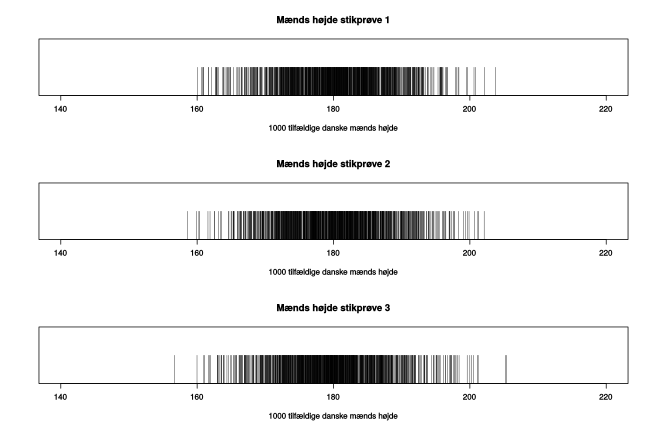
\includegraphics{_main_files/figure-latex/unnamed-chunk-7-1.pdf}

\hypertarget{detail-debet-card-forbrug-pa-island-millioner-isk.}{%
\subsection{Detail debet card forbrug på Island (millioner ISK).}\label{detail-debet-card-forbrug-pa-island-millioner-isk.}}

\begin{Shaded}
\begin{Highlighting}[]
\CommentTok{#Hent fpp pakken og load den}
\KeywordTok{plot}\NormalTok{(debitcards)}
\end{Highlighting}
\end{Shaded}

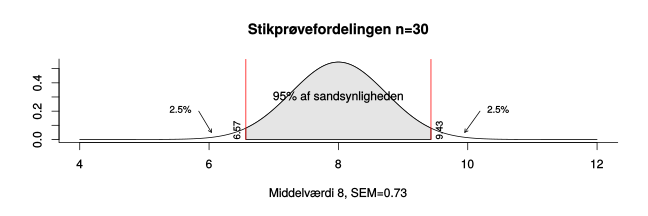
\includegraphics{_main_files/figure-latex/unnamed-chunk-9-1.pdf}

\begin{Shaded}
\begin{Highlighting}[]
\NormalTok{dldebitcards <-}\StringTok{ }\KeywordTok{diff}\NormalTok{(}\KeywordTok{log10}\NormalTok{(debitcards))}
\KeywordTok{plot}\NormalTok{(dldebitcards,}\DataTypeTok{ylab=}\StringTok{"Differenced Log (debitcards)"}\NormalTok{)}
\end{Highlighting}
\end{Shaded}

\includegraphics{_main_files/figure-latex/unnamed-chunk-10-1.pdf}

\begin{Shaded}
\begin{Highlighting}[]
\KeywordTok{require}\NormalTok{(forecast)}
\NormalTok{ARIMAfit =}\StringTok{ }\KeywordTok{auto.arima}\NormalTok{(}\KeywordTok{log10}\NormalTok{(debitcards), }\DataTypeTok{approximation=}\OtherTok{FALSE}\NormalTok{,}\DataTypeTok{trace=}\OtherTok{FALSE}\NormalTok{)}
\NormalTok{ARIMAfit}
\end{Highlighting}
\end{Shaded}

\begin{verbatim}
## Series: log10(debitcards) 
## ARIMA(2,1,0)(0,1,1)[12] 
## 
## Coefficients:
##           ar1      ar2     sma1
##       -0.7167  -0.4372  -0.8352
## s.e.   0.0761   0.0763   0.1085
## 
## sigma^2 estimated as 0.0004402:  log likelihood=343.95
## AIC=-679.9   AICc=-679.61   BIC=-668.05
\end{verbatim}

Nu kan vi forudsige kommende debetkort omsætning med modellen

\begin{Shaded}
\begin{Highlighting}[]
\KeywordTok{par}\NormalTok{(}\DataTypeTok{mfrow =} \KeywordTok{c}\NormalTok{(}\DecValTok{1}\NormalTok{,}\DecValTok{1}\NormalTok{))}
\NormalTok{pred =}\StringTok{ }\KeywordTok{predict}\NormalTok{(ARIMAfit, }\DataTypeTok{n.ahead =} \DecValTok{36}\NormalTok{)}
\KeywordTok{plot}\NormalTok{(debitcards,}\DataTypeTok{type=}\StringTok{'l'}\NormalTok{,}\DataTypeTok{xlim=}\KeywordTok{c}\NormalTok{(}\DecValTok{2000}\NormalTok{,}\DecValTok{2016}\NormalTok{),}\DataTypeTok{ylim=}\KeywordTok{c}\NormalTok{(}\DecValTok{1}\NormalTok{,}\DecValTok{40000}\NormalTok{),}\DataTypeTok{xlab =} \StringTok{'Year'}\NormalTok{,}\DataTypeTok{ylab =} \StringTok{'Debetcard usage'}\NormalTok{)}
\KeywordTok{lines}\NormalTok{(}\DecValTok{10}\OperatorTok{^}\NormalTok{(pred}\OperatorTok{$}\NormalTok{pred),}\DataTypeTok{col=}\StringTok{'blue'}\NormalTok{)}
\KeywordTok{lines}\NormalTok{(}\DecValTok{10}\OperatorTok{^}\NormalTok{(pred}\OperatorTok{$}\NormalTok{pred}\OperatorTok{+}\DecValTok{2}\OperatorTok{*}\NormalTok{pred}\OperatorTok{$}\NormalTok{se),}\DataTypeTok{col=}\StringTok{'orange'}\NormalTok{)}
\KeywordTok{lines}\NormalTok{(}\DecValTok{10}\OperatorTok{^}\NormalTok{(pred}\OperatorTok{$}\NormalTok{pred}\DecValTok{-2}\OperatorTok{*}\NormalTok{pred}\OperatorTok{$}\NormalTok{se),}\DataTypeTok{col=}\StringTok{'orange'}\NormalTok{)}
\end{Highlighting}
\end{Shaded}

\includegraphics{_main_files/figure-latex/unnamed-chunk-12-1.pdf}

Forudsagt brug af debetkort bliver:

\begin{Shaded}
\begin{Highlighting}[]
\DecValTok{10}\OperatorTok{^}\NormalTok{(pred}\OperatorTok{$}\NormalTok{pred)}
\end{Highlighting}
\end{Shaded}

\begin{verbatim}
##           Jan      Feb      Mar      Apr      May      Jun      Jul
## 2013 19717.77 19162.87 20436.29 20506.84 23262.14 23545.62 24292.86
## 2014 20701.39 20352.57 21886.85 21721.53 24745.18 25091.09 25806.49
## 2015 22017.60 21649.95 23281.85 23104.56 26321.98 26689.74 27450.29
##           Aug      Sep      Oct      Nov      Dec
## 2013 25544.16 22267.47 22543.80 22081.63 29090.93
## 2014 27175.65 23697.15 23970.40 23490.36 30947.83
## 2015 28907.08 25206.87 25497.43 24986.92 32919.46
\end{verbatim}

\hypertarget{forecast-aktiekurser}{%
\section{Forecast Aktiekurser}\label{forecast-aktiekurser}}

Man kan hente online aktiekurser med quantmod pakken installer denne med fx. pacman, vi skal også bruge pakken forecast som vi ligeledes henter. Vi henter nedenfor Google justeret lukkekurs til dato det er 6 søjle i GOOG matricen nedenfor. Vi kan se forecaste aktiekursen vha.

\begin{Shaded}
\begin{Highlighting}[]
\NormalTok{pacman}\OperatorTok{::}\KeywordTok{p_load}\NormalTok{(quantmod, forecast)}
\KeywordTok{getSymbols}\NormalTok{(}\StringTok{"GOOG"}\NormalTok{,}\DataTypeTok{from =} \StringTok{"2017-01-01"}\NormalTok{, }\DataTypeTok{to =} \KeywordTok{Sys.Date}\NormalTok{(),}\DataTypeTok{getSymbols.warning4.0=}\OtherTok{FALSE}\NormalTok{)}
\end{Highlighting}
\end{Shaded}

\begin{verbatim}
## [1] "GOOG"
\end{verbatim}

\begin{Shaded}
\begin{Highlighting}[]
\KeywordTok{plot}\NormalTok{(GOOG[,}\DecValTok{6}\NormalTok{],}\DataTypeTok{main =} \StringTok{"Google adj. close"}\NormalTok{)}
\end{Highlighting}
\end{Shaded}

\includegraphics{_main_files/figure-latex/unnamed-chunk-15-1.pdf}

\begin{Shaded}
\begin{Highlighting}[]
\NormalTok{agoog <-}\StringTok{ }\KeywordTok{auto.arima}\NormalTok{(GOOG[,}\DecValTok{6}\NormalTok{])}
\NormalTok{agoog}
\end{Highlighting}
\end{Shaded}

\begin{verbatim}
## Series: GOOG[, 6] 
## ARIMA(0,1,0) 
## 
## sigma^2 estimated as 227.3:  log likelihood=-2400.69
## AIC=4803.39   AICc=4803.4   BIC=4807.75
\end{verbatim}

\begin{Shaded}
\begin{Highlighting}[]
\NormalTok{fagoog <-}\StringTok{ }\KeywordTok{forecast}\NormalTok{(agoog)}
\NormalTok{fagoog}
\end{Highlighting}
\end{Shaded}

\begin{verbatim}
##     Point Forecast    Lo 80    Hi 80    Lo 95    Hi 95
## 583        1272.18 1252.860 1291.500 1242.633 1301.727
## 584        1272.18 1244.857 1299.503 1230.394 1313.966
## 585        1272.18 1238.717 1305.643 1221.003 1323.358
## 586        1272.18 1233.540 1310.820 1213.085 1331.275
## 587        1272.18 1228.979 1315.381 1206.110 1338.250
## 588        1272.18 1224.856 1319.504 1199.804 1344.556
## 589        1272.18 1221.064 1323.296 1194.005 1350.355
## 590        1272.18 1217.535 1326.825 1188.608 1355.753
## 591        1272.18 1214.220 1330.140 1183.538 1360.822
## 592        1272.18 1211.085 1333.275 1178.743 1365.617
\end{verbatim}

\begin{Shaded}
\begin{Highlighting}[]
\KeywordTok{plot}\NormalTok{(fagoog,}\DataTypeTok{main =} \StringTok{"Google adj. close"}\NormalTok{)}
\end{Highlighting}
\end{Shaded}

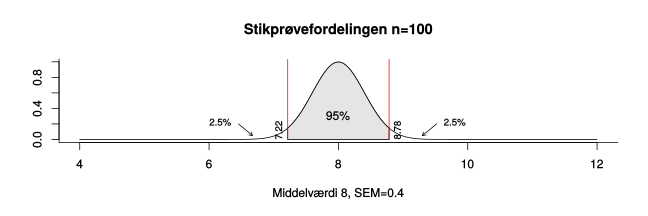
\includegraphics{_main_files/figure-latex/unnamed-chunk-16-1.pdf}

\begin{Shaded}
\begin{Highlighting}[]
\KeywordTok{getSymbols}\NormalTok{(}\StringTok{"GS"}\NormalTok{,}\DataTypeTok{from =} \StringTok{"2017-01-01"}\NormalTok{, }\DataTypeTok{to =} \KeywordTok{Sys.Date}\NormalTok{(),}\DataTypeTok{getSymbols.warning4.0=}\OtherTok{FALSE}\NormalTok{)}
\end{Highlighting}
\end{Shaded}

\begin{verbatim}
## [1] "GS"
\end{verbatim}

\begin{Shaded}
\begin{Highlighting}[]
\KeywordTok{plot}\NormalTok{(GS[,}\DecValTok{6}\NormalTok{],}\DataTypeTok{main =} \StringTok{"Goldman Sachs adj. close"}\NormalTok{)}
\end{Highlighting}
\end{Shaded}

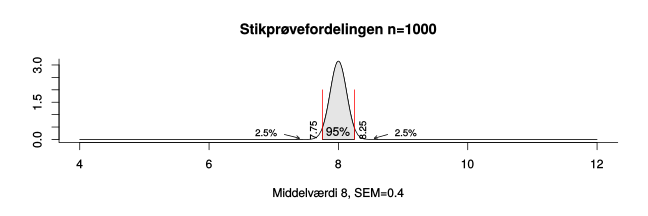
\includegraphics{_main_files/figure-latex/unnamed-chunk-17-1.pdf}

\begin{Shaded}
\begin{Highlighting}[]
\NormalTok{ags <-}\StringTok{ }\KeywordTok{auto.arima}\NormalTok{(GS[,}\DecValTok{6}\NormalTok{])}
\NormalTok{ags}
\end{Highlighting}
\end{Shaded}

\begin{verbatim}
## Series: GS[, 6] 
## ARIMA(0,1,0) 
## 
## sigma^2 estimated as 10.68:  log likelihood=-1512.31
## AIC=3026.62   AICc=3026.62   BIC=3030.98
\end{verbatim}

\begin{Shaded}
\begin{Highlighting}[]
\NormalTok{fags <-}\StringTok{ }\KeywordTok{forecast}\NormalTok{(ags)}
\NormalTok{fags}
\end{Highlighting}
\end{Shaded}

\begin{verbatim}
##     Point Forecast    Lo 80    Hi 80    Lo 95    Hi 95
## 583         203.08 198.8926 207.2674 196.6759 209.4841
## 584         203.08 197.1581 209.0019 194.0233 212.1367
## 585         203.08 195.8272 210.3328 191.9879 214.1722
## 586         203.08 194.7052 211.4548 190.2719 215.8881
## 587         203.08 193.7167 212.4433 188.7601 217.3999
## 588         203.08 192.8230 213.3370 187.3933 218.7667
## 589         203.08 192.0012 214.1588 186.1365 220.0235
## 590         203.08 191.2363 214.9237 184.9666 221.1934
## 591         203.08 190.5178 215.6422 183.8678 222.2922
## 592         203.08 189.8383 216.3217 182.8286 223.3314
\end{verbatim}

\begin{Shaded}
\begin{Highlighting}[]
\KeywordTok{plot}\NormalTok{(fags,}\DataTypeTok{main =} \StringTok{"Goldman Sachs adj. close"}\NormalTok{)}
\end{Highlighting}
\end{Shaded}

\includegraphics{_main_files/figure-latex/unnamed-chunk-17-2.pdf}

\begin{Shaded}
\begin{Highlighting}[]
\KeywordTok{getSymbols}\NormalTok{(}\StringTok{"DANSKE.CO"}\NormalTok{,}\DataTypeTok{from =} \StringTok{"2017-01-01"}\NormalTok{, }\DataTypeTok{to =} \KeywordTok{Sys.Date}\NormalTok{(),}\DataTypeTok{getSymbols.warning4.0=}\OtherTok{FALSE}\NormalTok{)}
\end{Highlighting}
\end{Shaded}

\begin{verbatim}
## [1] "DANSKE.CO"
\end{verbatim}

\begin{Shaded}
\begin{Highlighting}[]
\KeywordTok{plot}\NormalTok{(DANSKE.CO[,}\DecValTok{6}\NormalTok{],}\DataTypeTok{main =} \StringTok{"Danske Bank adj. close"}\NormalTok{)}
\end{Highlighting}
\end{Shaded}

\includegraphics{_main_files/figure-latex/unnamed-chunk-18-1.pdf}

\begin{Shaded}
\begin{Highlighting}[]
\NormalTok{addb <-}\StringTok{ }\KeywordTok{auto.arima}\NormalTok{(DANSKE.CO[,}\DecValTok{6}\NormalTok{])}
\NormalTok{addb}
\end{Highlighting}
\end{Shaded}

\begin{verbatim}
## Series: DANSKE.CO[, 6] 
## ARIMA(1,2,2) 
## 
## Coefficients:
##           ar1      ma1      ma2
##       -0.2609  -0.8131  -0.1748
## s.e.   0.3035   0.3082   0.3057
## 
## sigma^2 estimated as 6.441:  log likelihood=-1356.64
## AIC=2721.28   AICc=2721.35   BIC=2738.71
\end{verbatim}

\begin{Shaded}
\begin{Highlighting}[]
\NormalTok{faddb <-}\StringTok{ }\KeywordTok{forecast}\NormalTok{(addb)}
\NormalTok{faddb}
\end{Highlighting}
\end{Shaded}

\begin{verbatim}
##     Point Forecast    Lo 80    Hi 80    Lo 95    Hi 95
## 580       128.2108 124.9582 131.4633 123.2364 133.1851
## 581       128.1523 123.7194 132.5851 121.3728 134.9317
## 582       128.0335 122.6163 133.4508 119.7486 136.3185
## 583       127.9306 121.6758 134.1853 118.3648 137.4963
## 584       127.8235 120.8147 134.8323 117.1044 138.5425
## 585       127.7174 120.0158 135.4190 115.9388 139.4960
## 586       127.6111 119.2620 135.9603 114.8422 140.3800
## 587       127.5049 118.5437 136.4661 113.7999 141.2098
## 588       127.3986 117.8539 136.9433 112.8013 141.9960
## 589       127.2924 117.1877 137.3971 111.8385 142.7462
\end{verbatim}

\begin{Shaded}
\begin{Highlighting}[]
\KeywordTok{plot}\NormalTok{(faddb,}\DataTypeTok{main =} \StringTok{"Danske Bank adj. close"}\NormalTok{)}
\end{Highlighting}
\end{Shaded}

\includegraphics{_main_files/figure-latex/unnamed-chunk-18-2.pdf}

\begin{Shaded}
\begin{Highlighting}[]
\KeywordTok{getSymbols}\NormalTok{(}\StringTok{"BRK-A"}\NormalTok{,}\DataTypeTok{from =} \StringTok{"2000-01-01"}\NormalTok{, }\DataTypeTok{to =} \KeywordTok{Sys.Date}\NormalTok{(),}\DataTypeTok{getSymbols.warning4.0=}\OtherTok{FALSE}\NormalTok{)}
\end{Highlighting}
\end{Shaded}

\begin{verbatim}
## [1] "BRK-A"
\end{verbatim}

\begin{Shaded}
\begin{Highlighting}[]
\KeywordTok{plot}\NormalTok{(}\StringTok{`}\DataTypeTok{BRK-A}\StringTok{`}\NormalTok{[,}\DecValTok{6}\NormalTok{],}\DataTypeTok{main =} \StringTok{"Berkshire adj. close"}\NormalTok{)}
\end{Highlighting}
\end{Shaded}

\includegraphics{_main_files/figure-latex/unnamed-chunk-19-1.pdf}

\begin{Shaded}
\begin{Highlighting}[]
\NormalTok{aberkshire <-}\StringTok{ }\KeywordTok{auto.arima}\NormalTok{(}\StringTok{`}\DataTypeTok{BRK-A}\StringTok{`}\NormalTok{[,}\DecValTok{6}\NormalTok{])}
\NormalTok{aberkshire}
\end{Highlighting}
\end{Shaded}

\begin{verbatim}
## Series: `BRK-A`[, 6] 
## ARIMA(3,1,4) with drift 
## 
## Coefficients:
##          ar1      ar2     ar3      ma1     ma2      ma3      ma4    drift
##       0.9581  -0.8520  0.4078  -0.9895  0.8649  -0.4151  -0.0742  53.6558
## s.e.  0.4050   0.7223  0.4820   0.4055  0.7413   0.5257   0.0519  20.8218
## 
## sigma^2 estimated as 3341081:  log likelihood=-43377.2
## AIC=86772.4   AICc=86772.44   BIC=86830.8
\end{verbatim}

\begin{Shaded}
\begin{Highlighting}[]
\NormalTok{faberkshire <-}\StringTok{ }\KeywordTok{forecast}\NormalTok{(aberkshire)}
\NormalTok{faberkshire}
\end{Highlighting}
\end{Shaded}

\begin{verbatim}
##      Point Forecast    Lo 80    Hi 80    Lo 95    Hi 95
## 4860       320636.1 318293.6 322978.6 317053.6 324218.6
## 4861       320499.4 317238.1 323760.7 315511.7 325487.1
## 4862       320499.6 316549.4 324449.8 314458.3 326540.9
## 4863       320307.1 315767.9 324846.3 313365.0 327249.2
## 4864       320092.8 315102.5 325083.1 312460.8 327724.8
## 4865       320077.6 314739.7 325415.6 311914.0 328241.3
## 4866       320193.3 314538.8 325847.9 311545.4 328841.2
## 4867       320255.7 314283.1 326228.3 311121.4 329390.0
## 4868       320236.8 313960.0 326513.7 310637.2 329836.4
## 4869       320238.8 313687.5 326790.2 310219.5 330258.2
\end{verbatim}

\begin{Shaded}
\begin{Highlighting}[]
\KeywordTok{plot}\NormalTok{(faberkshire,}\DataTypeTok{main =} \StringTok{"Berkshire adj. close"}\NormalTok{)}
\end{Highlighting}
\end{Shaded}

\includegraphics{_main_files/figure-latex/unnamed-chunk-19-2.pdf}

\hypertarget{aktieafkast}{%
\section{Aktieafkast}\label{aktieafkast}}

I Quantmod pakken ligger også mulighed for at beregne fx. dagligt, ugentligt afkast, dette gør vi vha. funktionen ``periodReturn''.

\begin{Shaded}
\begin{Highlighting}[]
\KeywordTok{getSymbols}\NormalTok{(}\StringTok{"AAPL"}\NormalTok{,}\DataTypeTok{src=}\StringTok{'yahoo'}\NormalTok{)}
\end{Highlighting}
\end{Shaded}

\begin{verbatim}
## [1] "AAPL"
\end{verbatim}

\begin{Shaded}
\begin{Highlighting}[]
\NormalTok{apple <-}\StringTok{ }\KeywordTok{periodReturn}\NormalTok{(}\StringTok{`}\DataTypeTok{AAPL}\StringTok{`}\NormalTok{,}\DataTypeTok{period=}\StringTok{'yearly'}\NormalTok{,}\DataTypeTok{subset=}\StringTok{'2003::'}\NormalTok{)  }\CommentTok{# Årligt Afkast 2003 til i dag}
\KeywordTok{plot}\NormalTok{(apple, }\DataTypeTok{main =} \StringTok{"Apple årligt afkast siden 2007"}\NormalTok{)}
\end{Highlighting}
\end{Shaded}

\includegraphics{_main_files/figure-latex/unnamed-chunk-20-1.pdf}

\begin{Shaded}
\begin{Highlighting}[]
\KeywordTok{auto.arima}\NormalTok{(apple)}
\end{Highlighting}
\end{Shaded}

\begin{verbatim}
## Series: apple 
## ARIMA(1,0,0) with non-zero mean 
## 
## Coefficients:
##           ar1    mean
##       -0.5894  0.3165
## s.e.   0.2455  0.0783
## 
## sigma^2 estimated as 0.2222:  log likelihood=-7.8
## AIC=21.59   AICc=24.26   BIC=23.29
\end{verbatim}

\begin{Shaded}
\begin{Highlighting}[]
\KeywordTok{getSymbols}\NormalTok{(}\StringTok{"BRK-A"}\NormalTok{,}\DataTypeTok{src=}\StringTok{'yahoo'}\NormalTok{)}
\end{Highlighting}
\end{Shaded}

\begin{verbatim}
## [1] "BRK-A"
\end{verbatim}

\begin{Shaded}
\begin{Highlighting}[]
\NormalTok{berkshire <-}\StringTok{ }\KeywordTok{periodReturn}\NormalTok{(}\StringTok{`}\DataTypeTok{BRK-A}\StringTok{`}\NormalTok{,}\DataTypeTok{period=}\StringTok{'yearly'}\NormalTok{,}\DataTypeTok{subset=}\StringTok{'2003::'}\NormalTok{)}
\KeywordTok{plot}\NormalTok{(berkshire, }\DataTypeTok{main =} \StringTok{"Berkshire årligt afkast siden 2007"}\NormalTok{)}
\end{Highlighting}
\end{Shaded}

\includegraphics{_main_files/figure-latex/unnamed-chunk-21-1.pdf}

\begin{Shaded}
\begin{Highlighting}[]
\KeywordTok{auto.arima}\NormalTok{(berkshire)}
\end{Highlighting}
\end{Shaded}

\begin{verbatim}
## Series: berkshire 
## ARIMA(0,0,0) with non-zero mean 
## 
## Coefficients:
##         mean
##       0.1023
## s.e.  0.0501
## 
## sigma^2 estimated as 0.0353:  log likelihood=3.81
## AIC=-3.62   AICc=-2.42   BIC=-2.49
\end{verbatim}

\hypertarget{arima-opsamling-video}{%
\subsection{ARIMA opsamling video}\label{arima-opsamling-video}}

\hypertarget{deskriptiv-statistik}{%
\chapter{Deskriptiv statistik}\label{deskriptiv-statistik}}

\hypertarget{Sentry_noJS}{}
Sentry Page Protection

\hypertarget{Sentry_redirecting}{}
Please Wait\ldots{}

\hypertarget{videoer-teori}{%
\section{Videoer teori}\label{videoer-teori}}

\hypertarget{introduktion}{%
\subsubsection{Introduktion}\label{introduktion}}

\hypertarget{data}{%
\subsubsection{Data}\label{data}}

\hypertarget{deskriptiv-statistik-1}{%
\subsubsection{Deskriptiv statistik}\label{deskriptiv-statistik-1}}

\hypertarget{fraktiler}{%
\subsubsection{Fraktiler}\label{fraktiler}}

\hypertarget{skvhed}{%
\subsubsection{Skævhed}\label{skvhed}}

\hypertarget{kurtosis}{%
\subsubsection{Kurtosis}\label{kurtosis}}

\hypertarget{sandsynligheder}{%
\subsubsection{Sandsynligheder}\label{sandsynligheder}}

\hypertarget{normalfordelingen}{%
\subsubsection{Normalfordelingen}\label{normalfordelingen}}

\hypertarget{konfidensintervaller-normalfordelingen}{%
\subsubsection{Konfidensintervaller normalfordelingen}\label{konfidensintervaller-normalfordelingen}}

\hypertarget{normalfraktildiagram}{%
\subsubsection{Normalfraktildiagram}\label{normalfraktildiagram}}

\hypertarget{stikprvefordelingen}{%
\subsubsection{Stikprøvefordelingen}\label{stikprvefordelingen}}

\hypertarget{stikprvefordelingen-2}{%
\subsubsection{Stikprøvefordelingen 2}\label{stikprvefordelingen-2}}

\hypertarget{parameter-estimat}{%
\subsubsection{Parameter-estimat}\label{parameter-estimat}}

\hypertarget{t-fordelingen}{%
\subsubsection{t-fordelingen}\label{t-fordelingen}}

\hypertarget{konfidensinterval-middelvrdien}{%
\subsubsection{Konfidensinterval middelværdien}\label{konfidensinterval-middelvrdien}}

\hypertarget{fejlmargin}{%
\subsubsection{Fejlmargin}\label{fejlmargin}}

\hypertarget{hypotesetest-middelvrdi}{%
\subsubsection{Hypotesetest middelværdi}\label{hypotesetest-middelvrdi}}

\hypertarget{liner-regression}{%
\subsubsection{Lineær regression}\label{liner-regression}}

\hypertarget{liner-regression-forudstninger}{%
\subsubsection{Lineær regression forudsætninger}\label{liner-regression-forudstninger}}

\hypertarget{goodness-of-fit-test}{%
\subsubsection{Goodness of fit test}\label{goodness-of-fit-test}}

\hypertarget{chi-i-anden-test}{%
\subsection{Chi i anden test}\label{chi-i-anden-test}}

\hypertarget{chi-i-anden-test-2}{%
\subsection{Chi i anden test 2}\label{chi-i-anden-test-2}}

\hypertarget{anova}{%
\subsection{Anova}\label{anova}}

\hypertarget{freestat-fin}{%
\section{Freestat FIN}\label{freestat-fin}}

\hypertarget{mindmap-hypoteser}{%
\subsubsection{Mindmap hypoteser}\label{mindmap-hypoteser}}

\hypertarget{beskrivende-statistik-freestat}{%
\subsubsection{Beskrivende statistik Freestat}\label{beskrivende-statistik-freestat}}

\hypertarget{middelvrdi-standardafvigelse-ki}{%
\subsubsection{Middelværdi standardafvigelse KI}\label{middelvrdi-standardafvigelse-ki}}

\hypertarget{middelvrdi-test}{%
\subsubsection{Middelværdi test}\label{middelvrdi-test}}

\hypertarget{middelvrdi-fejlmargin}{%
\subsubsection{Middelværdi fejlmargin}\label{middelvrdi-fejlmargin}}

\hypertarget{standardafvigelse-test}{%
\subsubsection{Standardafvigelse test}\label{standardafvigelse-test}}

\hypertarget{andel-test-og-ki}{%
\subsubsection{1 Andel test og KI}\label{andel-test-og-ki}}

\hypertarget{andel-fejlmargin-og-fpc}{%
\subsubsection{1 Andel fejlmargin og FPC}\label{andel-fejlmargin-og-fpc}}

\hypertarget{fpc-endelig-populations-korrektion-og-z-test}{%
\subsubsection{FPC endelig populations korrektion og z-test}\label{fpc-endelig-populations-korrektion-og-z-test}}

\hypertarget{andel-test-og-ki-1}{%
\subsubsection{1 Andel test og KI}\label{andel-test-og-ki-1}}

\hypertarget{andel-fejlmargin-og-fpc-1}{%
\subsubsection{1 Andel fejlmargin og FPC}\label{andel-fejlmargin-og-fpc-1}}

\hypertarget{andele}{%
\subsubsection{2 Andele}\label{andele}}

\hypertarget{middelvrdier}{%
\subsubsection{2 Middelværdier}\label{middelvrdier}}

\hypertarget{parret-t-test}{%
\subsubsection{Parret t-test}\label{parret-t-test}}

\hypertarget{korrelation}{%
\subsubsection{Korrelation}\label{korrelation}}

\hypertarget{simpel-liner-regression}{%
\subsubsection{Simpel lineær regression}\label{simpel-liner-regression}}

\hypertarget{simpel-liner-regression-pi-og-ki}{%
\subsubsection{Simpel lineær regression PI og KI}\label{simpel-liner-regression-pi-og-ki}}

\hypertarget{multipel-liner-regression}{%
\subsubsection{Multipel lineær regression}\label{multipel-liner-regression}}

\hypertarget{dummy-variable}{%
\subsubsection{Dummy variable}\label{dummy-variable}}

\hypertarget{multipel-liner-regression-forudsagt-vrdi}{%
\subsubsection{Multipel lineær regression forudsagt værdi}\label{multipel-liner-regression-forudsagt-vrdi}}

\hypertarget{anova-variansanalyse}{%
\subsubsection{ANOVA variansanalyse}\label{anova-variansanalyse}}

\hypertarget{eksamensvideoer}{%
\section{Eksamensvideoer}\label{eksamensvideoer}}

\begin{center}\rule{0.5\linewidth}{\linethickness}\end{center}

\begin{center}\rule{0.5\linewidth}{\linethickness}\end{center}

\begin{center}\rule{0.5\linewidth}{\linethickness}\end{center}

\hypertarget{eksamen-statistik-2-timer-2017-9-5}{%
\subsubsection{Eksamen statistik 2 timer 2017 9 5}\label{eksamen-statistik-2-timer-2017-9-5}}

\href{https://www.dropbox.com/s/3gd6mcocowe8glq/2017\%209\%20Statistik\%20Fin.pdf?dl=1}{2017 9 5 Opgave}
\href{https://www.dropbox.com/s/y4p8j90wjbzhtb3/2017\%209\%20statistik\%20Data\%202.RE.xlsx?dl=1}{2017 9 5 Data}
\href{https://www.dropbox.com/s/wruqocv7g0fvkob/2017\%209\%20Statistik\%20Fin\%20opg\%201\%20og\%203\%20l\%C3\%B8sning\%20skabelon\%20Freestat\%20.docx?dl=1}{2017 9 5 Løsningsforslag}

\hypertarget{opgave-1-1-normalfraktildiagram}{%
\paragraph{Opgave 1 1 Normalfraktildiagram}\label{opgave-1-1-normalfraktildiagram}}

\hypertarget{opgave-1-2-test-middel}{%
\paragraph{Opgave 1 2 Test middel}\label{opgave-1-2-test-middel}}

\hypertarget{opgave-1-3-varianshomogenitet}{%
\paragraph{Opgave 1 3 Varianshomogenitet}\label{opgave-1-3-varianshomogenitet}}

\hypertarget{opgave-1-4-test-af-2-middelvrdier}{%
\paragraph{Opgave 1 4 Test af 2 middelværdier}\label{opgave-1-4-test-af-2-middelvrdier}}

\hypertarget{opgave-1-5-konfidensinterval-for-forskellen-af-middelvrdier}{%
\paragraph{Opgave 1 5 Konfidensinterval for forskellen af middelværdier}\label{opgave-1-5-konfidensinterval-for-forskellen-af-middelvrdier}}

\hypertarget{opgave-3-1-test-af-andel}{%
\paragraph{Opgave 3 1 Test af andel}\label{opgave-3-1-test-af-andel}}

\hypertarget{opgave-3-2-konfidensinterval-for-middelvrdi}{%
\paragraph{Opgave 3 2 Konfidensinterval for middelværdi}\label{opgave-3-2-konfidensinterval-for-middelvrdi}}

\begin{center}\rule{0.5\linewidth}{\linethickness}\end{center}

\begin{center}\rule{0.5\linewidth}{\linethickness}\end{center}

\begin{center}\rule{0.5\linewidth}{\linethickness}\end{center}

\begin{center}\rule{0.5\linewidth}{\linethickness}\end{center}

\begin{center}\rule{0.5\linewidth}{\linethickness}\end{center}

\begin{center}\rule{0.5\linewidth}{\linethickness}\end{center}

\hypertarget{eksamen-statistik-2-timer-2016-8-10}{%
\subsubsection{Eksamen statistik 2 timer 2016 8 10}\label{eksamen-statistik-2-timer-2016-8-10}}

\href{https://drive.google.com/uc?export=download\&id=0B1E7VnhxsDMlTy1NVjFBMDRLZFk}{2016 8 10 Opgave}
\href{https://drive.google.com/uc?export=download\&id=0B1E7VnhxsDMlcVdQUVFjUEp2SUE}{2016 8 10 Data}
\href{https://drive.google.com/uc?export=download\&id=0B1E7VnhxsDMlQnNjMk9XZDZKWUU}{2016 8 10 Løsningsforslag}

\hypertarget{opgave-1-liner-regression}{%
\paragraph{Opgave 1 Lineær regression}\label{opgave-1-liner-regression}}

\hypertarget{opgave-2-andele}{%
\paragraph{Opgave 2 Andele}\label{opgave-2-andele}}

\hypertarget{opgave-3-middelvrdier}{%
\paragraph{Opgave 3 Middelværdier}\label{opgave-3-middelvrdier}}

\hypertarget{opgave-4-teori-ki-punktestimat-testniveau}{%
\paragraph{Opgave 4 Teori KI, punktestimat, testniveau}\label{opgave-4-teori-ki-punktestimat-testniveau}}

\begin{center}\rule{0.5\linewidth}{\linethickness}\end{center}

\begin{center}\rule{0.5\linewidth}{\linethickness}\end{center}

\begin{center}\rule{0.5\linewidth}{\linethickness}\end{center}

\begin{center}\rule{0.5\linewidth}{\linethickness}\end{center}

\begin{center}\rule{0.5\linewidth}{\linethickness}\end{center}

\begin{center}\rule{0.5\linewidth}{\linethickness}\end{center}

\hypertarget{eksamen-statistik-2-timer-2015-8-7}{%
\subsubsection{Eksamen statistik 2 timer 2015 8 7}\label{eksamen-statistik-2-timer-2015-8-7}}

\href{https://www.dropbox.com/s/dwbpp3ykq17tbvb/2015\%208\%207\%201.reeksamen.pdf?dl=1}{2015 8 7 Opgave}
\href{https://www.dropbox.com/s/45d1xkhjp3c0owh/2015\%208\%207\%20Data.xlsx?dl=1}{2015 8 7 Data}
\href{https://www.dropbox.com/s/9nhbc21yth3si6o/2015\%208\%207\%20Freestat\%20skabelon\%20l\%C3\%B8sning.docx?dl=1}{2015 8 7 Løsningsforslag}

\hypertarget{opgave-1.1}{%
\paragraph{Opgave 1.1}\label{opgave-1.1}}

\hypertarget{opgave-1.2}{%
\paragraph{Opgave 1.2}\label{opgave-1.2}}

\hypertarget{opgave-1.3}{%
\paragraph{Opgave 1.3}\label{opgave-1.3}}

\hypertarget{opgave-1.4}{%
\paragraph{Opgave 1.4}\label{opgave-1.4}}

\hypertarget{opgave-1.5}{%
\paragraph{Opgave 1.5}\label{opgave-1.5}}

\hypertarget{opgave-2.1-og-2.2}{%
\paragraph{Opgave 2.1 og 2.2}\label{opgave-2.1-og-2.2}}

\hypertarget{opgave-2.3}{%
\paragraph{Opgave 2.3}\label{opgave-2.3}}

\hypertarget{opgave-3.1}{%
\paragraph{Opgave 3.1}\label{opgave-3.1}}

\hypertarget{opgave-3.2}{%
\paragraph{Opgave 3.2}\label{opgave-3.2}}

\hypertarget{opgave-3.3}{%
\paragraph{Opgave 3.3}\label{opgave-3.3}}

\begin{center}\rule{0.5\linewidth}{\linethickness}\end{center}

\begin{center}\rule{0.5\linewidth}{\linethickness}\end{center}

\begin{center}\rule{0.5\linewidth}{\linethickness}\end{center}

\begin{center}\rule{0.5\linewidth}{\linethickness}\end{center}

\begin{center}\rule{0.5\linewidth}{\linethickness}\end{center}

\begin{center}\rule{0.5\linewidth}{\linethickness}\end{center}

\hypertarget{eksamen-statistik-2-timer-2015-3-4}{%
\subsubsection{Eksamen statistik 2 timer 2015 3 4}\label{eksamen-statistik-2-timer-2015-3-4}}

\href{https://drive.google.com/file/d/0B1E7VnhxsDMlLVBMek5kWEhRZlU/view?usp=sharing}{2015 3 4 Opgave}
\href{https://drive.google.com/file/d/0B1E7VnhxsDMlX0p3Qk8wWlNxM28/view?usp=sharing}{2015 3 4 Data}
\href{https://drive.google.com/file/d/0B1E7VnhxsDMlWXNWTW55Sk94RDA/view?usp=sharing}{2015 3 4 Løsningsforslag}

\hypertarget{opgave-1-liner-regression-1}{%
\paragraph{Opgave 1 lineær regression}\label{opgave-1-liner-regression-1}}

\hypertarget{opgave-2-test-af-2-middelvrdier}{%
\paragraph{Opgave 2 Test af 2 middelværdier}\label{opgave-2-test-af-2-middelvrdier}}

\hypertarget{opgave-3-ki-andel-og-middel-test-af-middel}{%
\paragraph{Opgave 3 KI andel og middel, test af middel}\label{opgave-3-ki-andel-og-middel-test-af-middel}}

\hypertarget{opgave-4-2-andele}{%
\paragraph{Opgave 4 2 Andele}\label{opgave-4-2-andele}}

\hypertarget{eksamensvideoer-au-smartlearning}{%
\section{Eksamensvideoer AU Smartlearning}\label{eksamensvideoer-au-smartlearning}}

\begin{center}\rule{0.5\linewidth}{\linethickness}\end{center}

\begin{center}\rule{0.5\linewidth}{\linethickness}\end{center}

\begin{center}\rule{0.5\linewidth}{\linethickness}\end{center}

\hypertarget{konverter-eksamensopgaven-til-word}{%
\subsubsection{Konverter eksamensopgaven til Word}\label{konverter-eksamensopgaven-til-word}}

\begin{center}\rule{0.5\linewidth}{\linethickness}\end{center}

\begin{center}\rule{0.5\linewidth}{\linethickness}\end{center}

\begin{center}\rule{0.5\linewidth}{\linethickness}\end{center}

\hypertarget{eksamen-statistik-au-smartlearning-4-timer-2017-6}{%
\subsubsection{Eksamen statistik AU Smartlearning 4 timer 2017 6}\label{eksamen-statistik-au-smartlearning-4-timer-2017-6}}

\href{https://www.dropbox.com/s/dlgt1hnh6wu4aja/Statistik\%20eksamensopgave\%20juni\%202017\%20opgave\%202.pdf?dl=1}{2017 6 Eksamensopgave}
\href{https://www.dropbox.com/s/s0fl0lg2i2zk2hh/Eksamen\%202017\%20juni\%20opgave\%202\%20L\%C3\%98SNING.docx?dl=1}{2017 6 Løsningsforslag}

\hypertarget{opgave-2.1-normalfraktildiagram}{%
\paragraph{Opgave 2.1 Normalfraktildiagram}\label{opgave-2.1-normalfraktildiagram}}

\hypertarget{opgave-2.2-test-varians}{%
\paragraph{Opgave 2.2 Test varians}\label{opgave-2.2-test-varians}}

\hypertarget{opgave-2.3-test-middel}{%
\paragraph{Opgave 2.3 Test Middel}\label{opgave-2.3-test-middel}}

\hypertarget{opgave-2.4-test-ens-varianser}{%
\paragraph{Opgave 2.4 Test ens varianser}\label{opgave-2.4-test-ens-varianser}}

\hypertarget{opgave-2.5-test-to-middelvrdier}{%
\paragraph{Opgave 2.5 Test to middelværdier}\label{opgave-2.5-test-to-middelvrdier}}

\hypertarget{opgave-2.6-sandsynlighed-normalfordelingen}{%
\paragraph{Opgave 2.6 Sandsynlighed normalfordelingen}\label{opgave-2.6-sandsynlighed-normalfordelingen}}

\hypertarget{opgave-2.7-sandsynlighed-normalfordelingen}{%
\paragraph{Opgave 2.7 Sandsynlighed normalfordelingen}\label{opgave-2.7-sandsynlighed-normalfordelingen}}

\begin{center}\rule{0.5\linewidth}{\linethickness}\end{center}

\begin{center}\rule{0.5\linewidth}{\linethickness}\end{center}

\begin{center}\rule{0.5\linewidth}{\linethickness}\end{center}

\hypertarget{eksamen-statistik-4-timer-2016-1}{%
\subsubsection{Eksamen statistik 4 timer 2016 1}\label{eksamen-statistik-4-timer-2016-1}}

\href{https://www.dropbox.com/s/t1h9o0xnutneavu/AU\%20Statistik\%20eksamensopgave\%20-\%20januar\%202016.pdf?dl=1}{2016 1 Opgave}

\href{https://www.dropbox.com/s/vk2igqyofts6fes/AU\%20Statistik\%20eksamensopgave\%20-\%20januar\%202016\%20l\%C3\%B8sningsforslag.docx?dl=1}{2016 1 Løsningsforslag}

\hypertarget{au-januar-2016-opgave-1.1}{%
\paragraph{AU januar 2016 Opgave 1.1}\label{au-januar-2016-opgave-1.1}}

\hypertarget{au-januar-2016-opgave-1.2}{%
\paragraph{AU januar 2016 Opgave 1.2}\label{au-januar-2016-opgave-1.2}}

\hypertarget{au-januar-2016-opgave-1.3}{%
\paragraph{AU januar 2016 Opgave 1.3}\label{au-januar-2016-opgave-1.3}}

\hypertarget{au-januar-2016-opgave-1.4}{%
\paragraph{AU januar 2016 Opgave 1.4}\label{au-januar-2016-opgave-1.4}}

\hypertarget{au-januar-2016-opgave-1.5}{%
\paragraph{AU januar 2016 Opgave 1.5}\label{au-januar-2016-opgave-1.5}}

\hypertarget{au-januar-2016-opgave-2.1-og-2.2}{%
\paragraph{AU januar 2016 Opgave 2.1 og 2.2}\label{au-januar-2016-opgave-2.1-og-2.2}}

\hypertarget{au-januar-2016-opgave-3.1}{%
\paragraph{AU januar 2016 Opgave 3.1}\label{au-januar-2016-opgave-3.1}}

\hypertarget{au-januar-2016-opgave-3.2}{%
\paragraph{AU januar 2016 Opgave 3.2}\label{au-januar-2016-opgave-3.2}}

\hypertarget{au-januar-2016-opgave-3.3}{%
\paragraph{AU januar 2016 Opgave 3.3}\label{au-januar-2016-opgave-3.3}}

\hypertarget{au-januar-2016-opgave-3.4}{%
\paragraph{AU januar 2016 Opgave 3.4}\label{au-januar-2016-opgave-3.4}}

\hypertarget{au-januar-2016-opgave-4.1-og-4.2}{%
\paragraph{AU januar 2016 Opgave 4.1 og 4.2}\label{au-januar-2016-opgave-4.1-og-4.2}}

\begin{center}\rule{0.5\linewidth}{\linethickness}\end{center}

\begin{center}\rule{0.5\linewidth}{\linethickness}\end{center}

\begin{center}\rule{0.5\linewidth}{\linethickness}\end{center}

\hypertarget{eksamen-statistik-4-timer-2015-6}{%
\subsubsection{Eksamen statistik 4 timer 2015 6}\label{eksamen-statistik-4-timer-2015-6}}

\href{https://www.dropbox.com/s/lpyp894as98ho11/Smartlearning\%20AU\%202015\%206.pdf?dl=1}{2015 6 Opgave}
\href{https://www.dropbox.com/s/kf4avnc43qpz20d/2015\%206\%20AU\%20SMART\%20Vejledende.docx?dl=1}{2015 6 Løsningsforslag}

\hypertarget{opgave-1.1-eksamen-au-statistik-4-timer-2015-6}{%
\paragraph{Opgave 1.1 Eksamen AU statistik 4 timer 2015 6}\label{opgave-1.1-eksamen-au-statistik-4-timer-2015-6}}

\hypertarget{opgave-1.2-eksamen-au-statistik-4-timer-2015-6}{%
\paragraph{Opgave 1.2 Eksamen AU statistik 4 timer 2015 6}\label{opgave-1.2-eksamen-au-statistik-4-timer-2015-6}}

\hypertarget{opgave-1.3-eksamen-au-statistik-4-timer-2015-6}{%
\paragraph{Opgave 1.3 Eksamen AU statistik 4 timer 2015 6}\label{opgave-1.3-eksamen-au-statistik-4-timer-2015-6}}

\hypertarget{opgave-1.4-eksamen-au-statistik-4-timer-2015-6}{%
\paragraph{Opgave 1.4 Eksamen AU statistik 4 timer 2015 6}\label{opgave-1.4-eksamen-au-statistik-4-timer-2015-6}}

\hypertarget{opgave-1.5-eksamen-au-statistik-4-timer-2015-6}{%
\paragraph{Opgave 1.5 Eksamen AU statistik 4 timer 2015 6}\label{opgave-1.5-eksamen-au-statistik-4-timer-2015-6}}

\hypertarget{opgave-1.6-eksamen-au-statistik-4-timer-2015-6}{%
\paragraph{Opgave 1.6 Eksamen AU statistik 4 timer 2015 6}\label{opgave-1.6-eksamen-au-statistik-4-timer-2015-6}}

\hypertarget{opgave-1.7-eksamen-au-statistik-4-timer-2015-6}{%
\paragraph{Opgave 1.7 Eksamen AU statistik 4 timer 2015 6}\label{opgave-1.7-eksamen-au-statistik-4-timer-2015-6}}

\hypertarget{opgave-2.1-eksamen-au-statistik-4-timer-2015-6}{%
\paragraph{Opgave 2.1 Eksamen AU statistik 4 timer 2015 6}\label{opgave-2.1-eksamen-au-statistik-4-timer-2015-6}}

\hypertarget{opgave-2.2-og-2.3-eksamen-au-statistik-4-timer-2015-6}{%
\paragraph{Opgave 2.2 og 2.3 Eksamen AU statistik 4 timer 2015 6}\label{opgave-2.2-og-2.3-eksamen-au-statistik-4-timer-2015-6}}

\hypertarget{opgave-3.1-eksamen-au-statistik-4-timer-2015-6}{%
\paragraph{Opgave 3.1 Eksamen AU statistik 4 timer 2015 6}\label{opgave-3.1-eksamen-au-statistik-4-timer-2015-6}}

\hypertarget{opgave-3.2-og-3.3-eksamen-au-statistik-4-timer-2015-6}{%
\paragraph{Opgave 3.2 og 3.3 Eksamen AU statistik 4 timer 2015 6}\label{opgave-3.2-og-3.3-eksamen-au-statistik-4-timer-2015-6}}

\hypertarget{opgave-3.4-eksamen-au-statistik-4-timer-2015-6}{%
\paragraph{Opgave 3.4 Eksamen AU statistik 4 timer 2015 6}\label{opgave-3.4-eksamen-au-statistik-4-timer-2015-6}}

\hypertarget{opgave-4.1-eksamen-au-statistik-4-timer-2015-6}{%
\paragraph{Opgave 4.1 Eksamen AU statistik 4 timer 2015 6}\label{opgave-4.1-eksamen-au-statistik-4-timer-2015-6}}

\hypertarget{opgave-4.2-eksamen-au-statistik-4-timer-2015-6}{%
\paragraph{Opgave 4.2 Eksamen AU statistik 4 timer 2015 6}\label{opgave-4.2-eksamen-au-statistik-4-timer-2015-6}}

\hypertarget{opgave-4.3-eksamen-au-statistik-4-timer-2015-6}{%
\paragraph{Opgave 4.3 Eksamen AU statistik 4 timer 2015 6}\label{opgave-4.3-eksamen-au-statistik-4-timer-2015-6}}

\bibliography{book.bib,packages.bib}


\end{document}
